\documentclass[journal]{IEEEtran}
\usepackage[a5paper, margin=10mm, onecolumn]{geometry}
\usepackage[cmex10]{amsmath}
\usepackage{amssymb,amsfonts,amsthm}
\usepackage{gvv-book}
\usepackage{gvv}
\usepackage{hyperref}
\usepackage{physics}
\usepackage{gauss}

\begin{document}
\title{4.11.3}
\author{EE25BTECH11025 - Ganachari Vishwambhar}
\maketitle

\textbf{Question}:\\
Find the equation of the line passing through (2,-1,2) and (5,3,4) and the equation of the plane passing through (2,0,3), (1,1,5), and (3,2,4). Also, find their point of intersection.
\textbf{Solution: }\\

Let:
\begin{align}
    \vec{P}_1=\myvec{2\\-1\\2};
    \vec{P}_2=\myvec{5\\3\\4}\\
    \vec{A}=\myvec{2\\0\\3};\vec{B}=\myvec{1\\1\\5};\vec{C}=\myvec{3\\2\\4}    
\end{align}

Direction vector of the line:
\begin{align}
    \vec{m}=\vec{P}_2-\vec{P}_1=\myvec{5\\3\\4}-\myvec{2\\-1\\2}=\myvec{3\\4\\2}
\end{align}

Vector form of the line can be written as:
\begin{align}
    \vec{x}=\vec{P}_1+\kappa\vec{m}
\end{align}

Vector form of the line can be written as:
\begin{align}
    \myvec{\vec{A}&\vec{B}&\vec{C}}^\top\vec{n}=\vec{1}\\
    \myvec{2&0&3\\1&1&5\\3&2&4}\vec{n}=\myvec{1\\1\\1}
\end{align}
Augmented matrix can be written as:
\begin{align}
    \augvec{3}{1}{2&0&3&1\\1&1&5&1\\3&2&4&1}R_2 \leftrightarrow R_1
    \augvec{3}{1}{1&1&5&1\\2&0&3&1\\3&2&4&1}\frac{R_2\rightarrow R_2-2R_1}{R_3\rightarrow R_3-3R_1}\\
    \augvec{3}{1}{1&1&5&1\\0&-2&-7&-1\\0&-1&-11&-2}\frac{R_2\leftrightarrow R_3}{R_2\rightarrow-R_2}\augvec{3}{1}{1&1&5&1\\0&1&11&2\\0&-2&-7&-1}\\
    \frac{R_1\rightarrow R_1-R_2}{R_3\rightarrow R_3+2R_2}\augvec{3}{1}{1&0&-6&-1\\0&1&11&2\\0&0&15&3}R_3\rightarrow \frac{1}{15}R_3\\
    \augvec{3}{1}{1&0&-6&-1\\0&1&11&2\\0&0&1&\frac{1}{5}}\frac{R_1\rightarrow R_1+6R_3}{R_2\rightarrow R_2-11R_3}\augvec{3}{1}{1&0&0&\frac{1}{5}\\0&1&0&\frac{-1}{5}\\0&0&1&\frac{1}{5}}
\end{align}

Therefore, the plane equation is:
\begin{align}
    \myvec{1&-1&1}\vec{x}=5\\
    \vec{n}^\top\vec{x}=c
\end{align}

Substituting (4) in (11):
\begin{align}
    \vec{n}^\top\myvec{\vec{P}_1+\kappa\vec{m}}=c\\
    (\vec{n}^\top\vec{P}_1)+(\kappa\vec{n}^\top\vec{m})=c\\
    \kappa=\frac{c-(\vec{n}^\top\vec{P}_1)}{\vec{n}^\top\vec{m}}
\end{align}

The point of intersection is (from(4)):
\begin{align}
    \vec{x}=\vec{P}_1+\brak{\frac{c-(\vec{n}^\top\vec{P}_1)}{\vec{n}^\top\vec{m}}}\vec{m}
\end{align}

Substituting the values from (11), (1) and (3):
\begin{align}
    \vec{x}=\myvec{2\\-1\\2}+\brak{\frac{0}{-3}}\myvec{3&4&2}\\
    \vec{x}=\myvec{2\\-1\\2}
\end{align}

\begin{figure}[h!]
   \centering
   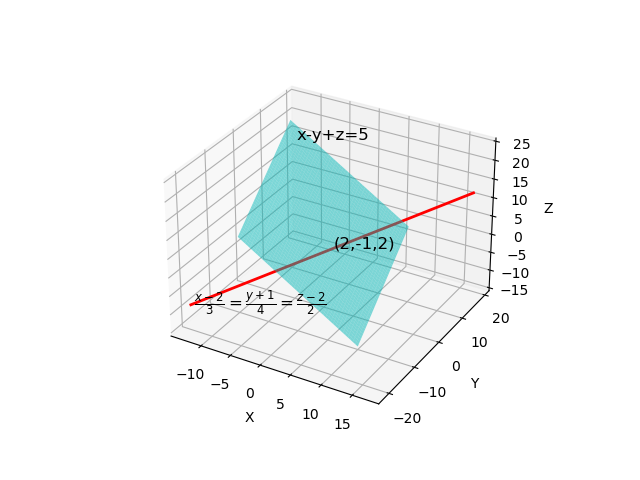
\includegraphics[width=0.7\linewidth]{figs/plot.png}
   \caption{Plot of the given plane and line}
   \label{}
\end{figure}
\end{document}  